\subsection{Supplemental:  Cross-section Ratios to GENIE}
\label{sec:appendixA}
Ratios between the data and the default tuned GENIE simulation are shown in the plots in this section.  The ratios between the various model choices in different generators and the default tuned GENIE simulation are also shown in this section.  The descriptions of the different model choices for each generator are described in Tab.~\ref{tab:generators}.  In many kinematic regions the measurement uncertainties are considerably smaller than the variations between different models, especially for the heavier nuclear targets and for scintillator where the statistics are the highest.  
\begin{figure}
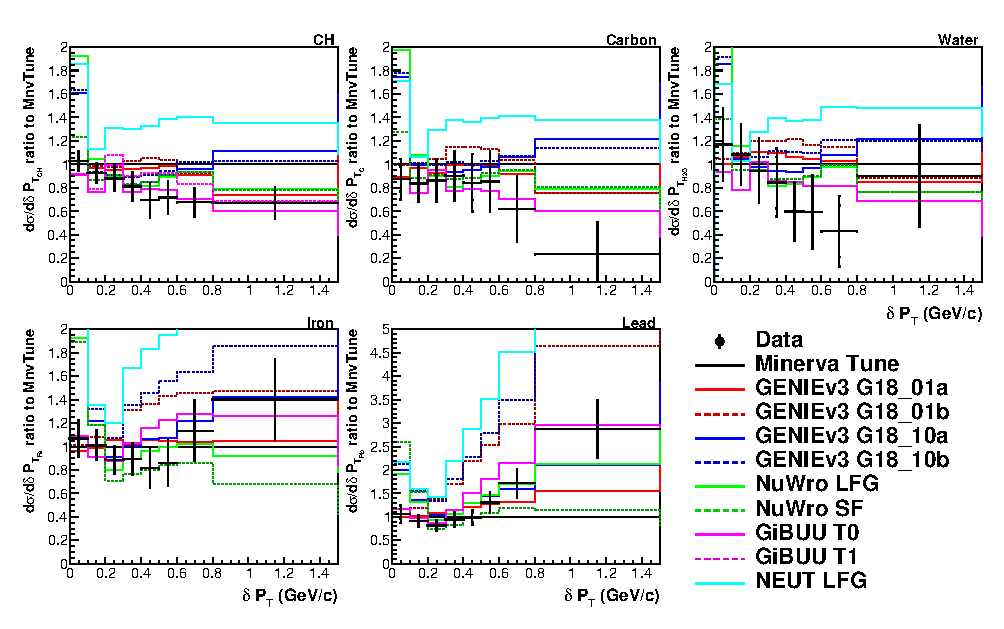
\includegraphics[width=\linewidth]{Figures/gencompare_ratio/mnvratio_dpt_fine.eps}
    \caption[\tkidelta \ cross-section comparison to the MINERvA tune for multiple targets ]{Ratio of absolute cross section measurements to the MINERvA tune for different targets as a function of \tkidelta\ and ratios of different model predictions to the MINERvA tune. 
    }
    \label{fig:models_dpt_rat}
\end{figure}
\begin{figure}
    \centering
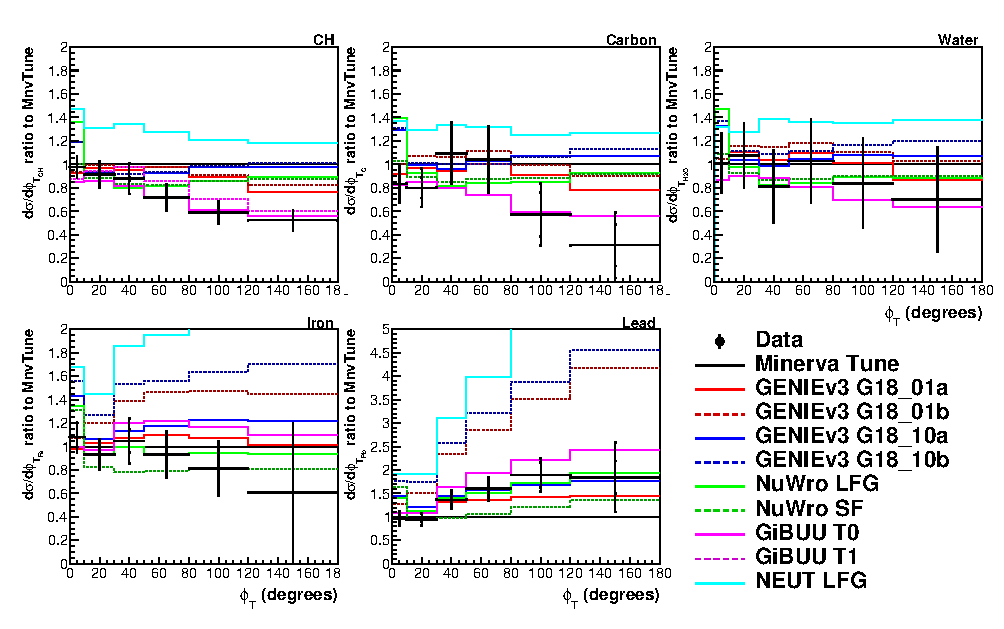
\includegraphics[width=\linewidth]{Figures/gencompare_ratio/mnvratio_phi.eps}
    \caption[\tkicoplanar \ cross-section ratio to the MINERvA tune for multiple targets ]{Ratio of absolute cross section measurements to the MINERvA tune for different targets as a function of  \tkicoplanar\ and ratios of different model predictions to the MINERvA tune.}
    \label{fig:models_coplan_rat}
\end{figure}
\begin{figure}
    \centering
    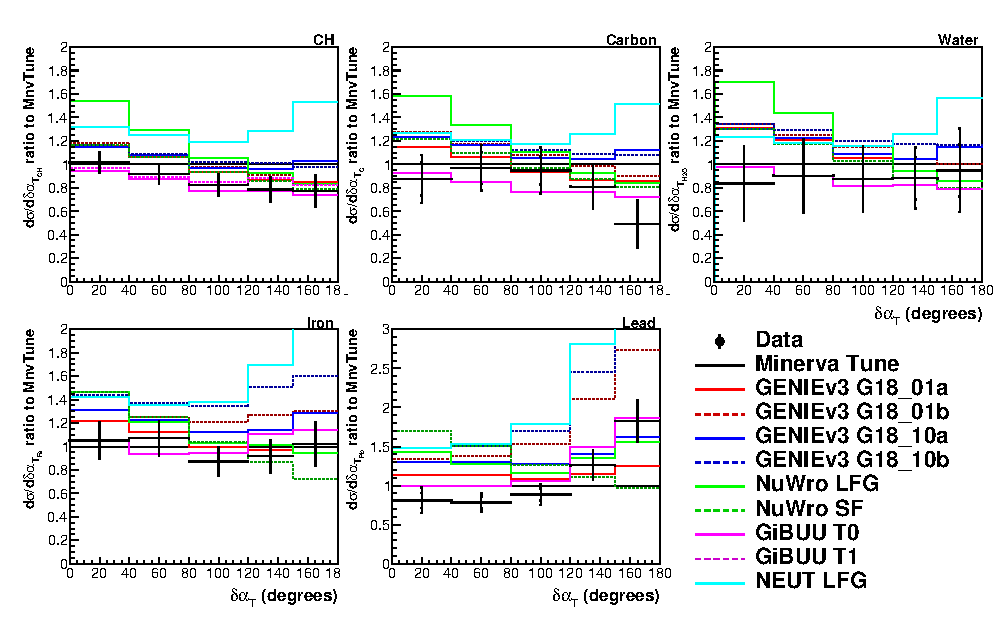
\includegraphics[width=\linewidth]{Figures/gencompare_ratio/mnvratio_alpha.eps}
    \caption[\tkialpha \ cross-section comparison for multiple targets ]{Ratio of absolute cross section measurements to the MINERvA tune for different targets as a function of  \tkialpha\ and ratios of different model predictions to the MINERvA tune.}
    \label{fig:models_alphat_rat}
\end{figure}
\begin{figure}
    \centering
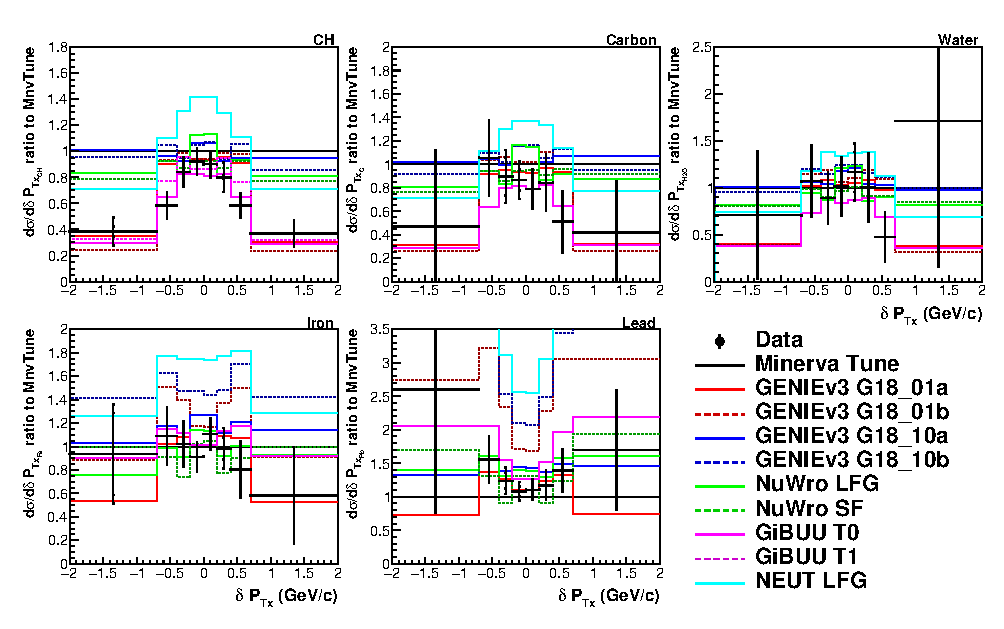
\includegraphics[width=\linewidth]{Figures/gencompare_ratio/mnvratio_dptx.eps}
    \caption{Ratio of absolute cross section measurements to the MINERvA tune for different targets as a function of  \tkidptx\ and ratios of different model predictions to the MINERvA tune.}
    \label{fig:models_dptx_rat}
\end{figure}
\begin{figure}
    \centering
    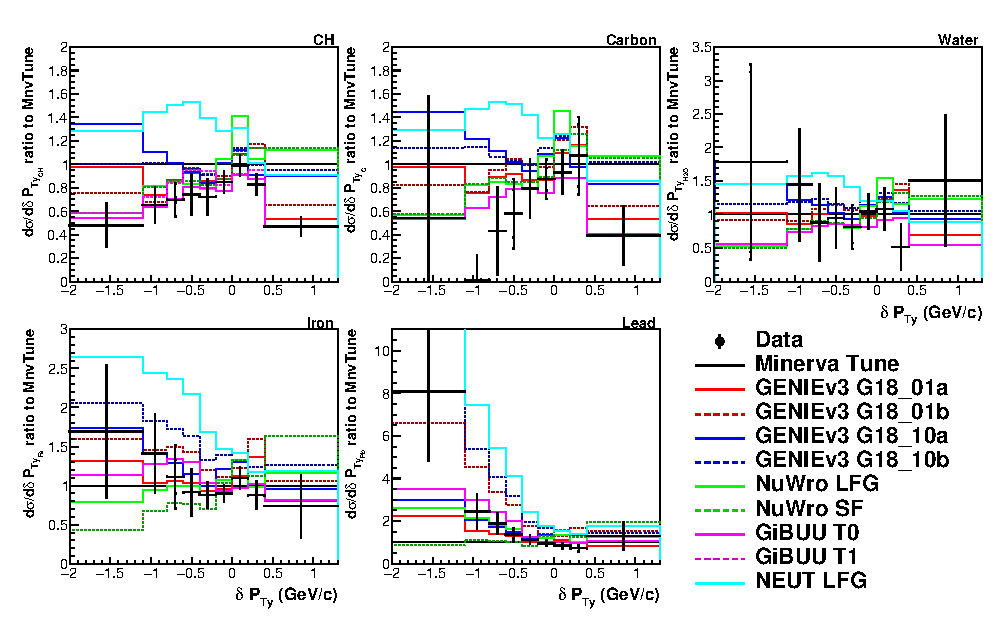
\includegraphics[width=\linewidth]{Figures/gencompare_ratio/mnvratio_dpty.eps}
     \caption{Ratio of absolute cross section measurements to the MINERvA tune for different targets as a function of  \tkidpty\ and ratios of different model predictions to the MINERvA tune. }
    \label{fig:models_dpty_rat}
\end{figure}
\begin{figure}
    \centering
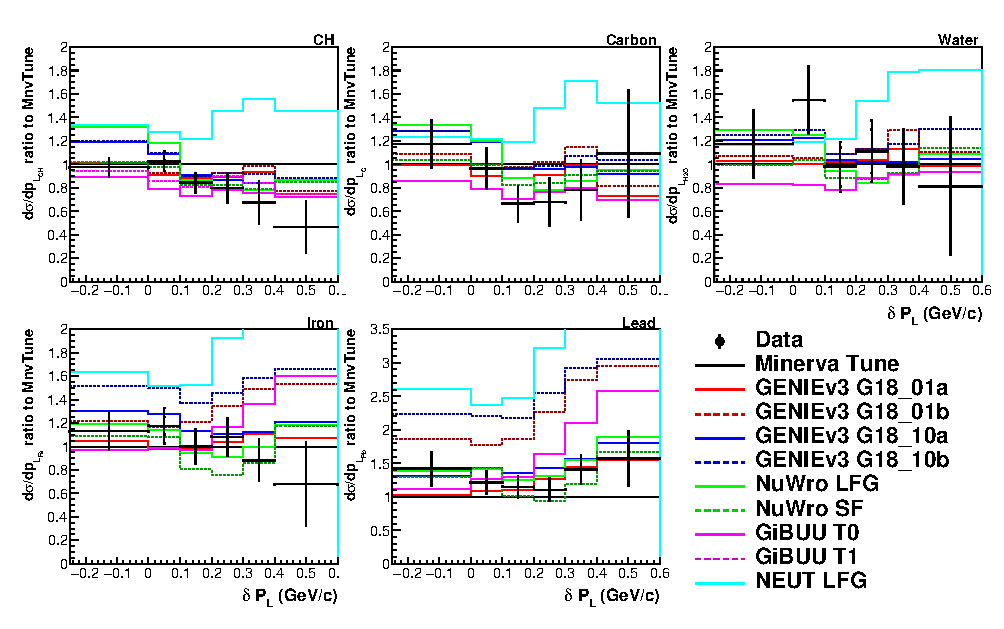
\includegraphics[width=\linewidth]{Figures/gencompare_ratio/mnvratio_pl.eps}
    \caption{Ratio of absolute cross section measurements to the MINERvA tune for different targets as a function of  \tkipl\ and ratios of different model predictions to the MINERvA tune.}
    \label{fig:models_pl_rat}
\end{figure}
\begin{figure}
    \centering            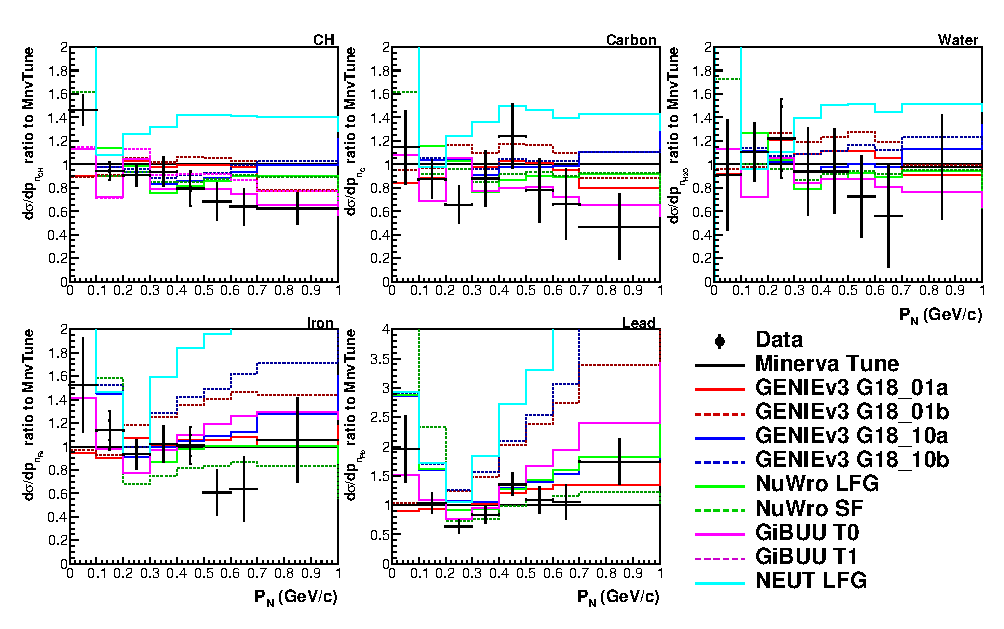
\includegraphics[width=\linewidth]{Figures/gencompare_ratio/mnvratio_pn.eps}
    \caption{Ratio of absolute cross section measurements to the MINERvA tune for different targets as a function of  \tkipn\ and ratios of different model predictions to the MINERvA tune.}
    \label{fig:models_pn_rat}
\end{figure}
\begin{figure}
    \centering
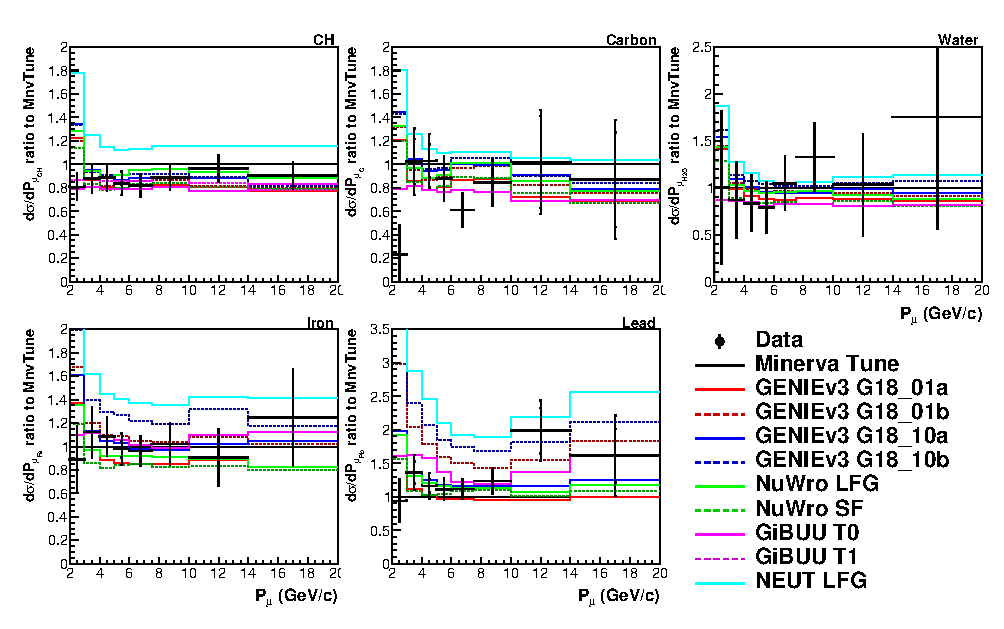
\includegraphics[width=\linewidth]{Figures/gencompare_ratio/mnvratio_muon_p.eps}
    \caption{Ratio of absolute cross section measurements to the MINERvA tune for different targets as a function of  P$_\mu$ and ratios of different model predictions to the MINERvA tune.}
    \label{fig:models_muon_p_rat}
\end{figure}
\begin{figure}
    \centering
    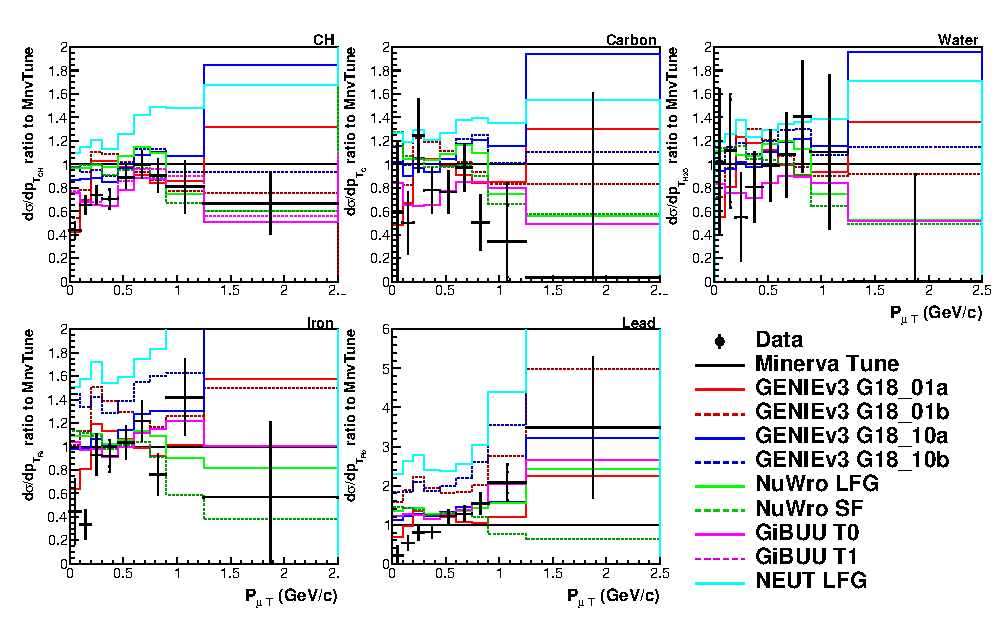
\includegraphics[width=\linewidth]{Figures/gencompare_ratio/mnvratio_muon_pt.eps}
    \caption[\tkiptmu \ cross-section comparison for multiple targets ]{Ratio of absolute cross section measurements to the MINERvA tune for different targets as a function of  \tkiptmu\ and ratios of different model predictions to the MINERvA tune.}
    \label{Figure:Gencompare_ptmu_rat}
\end{figure}
\begin{figure}
    \centering
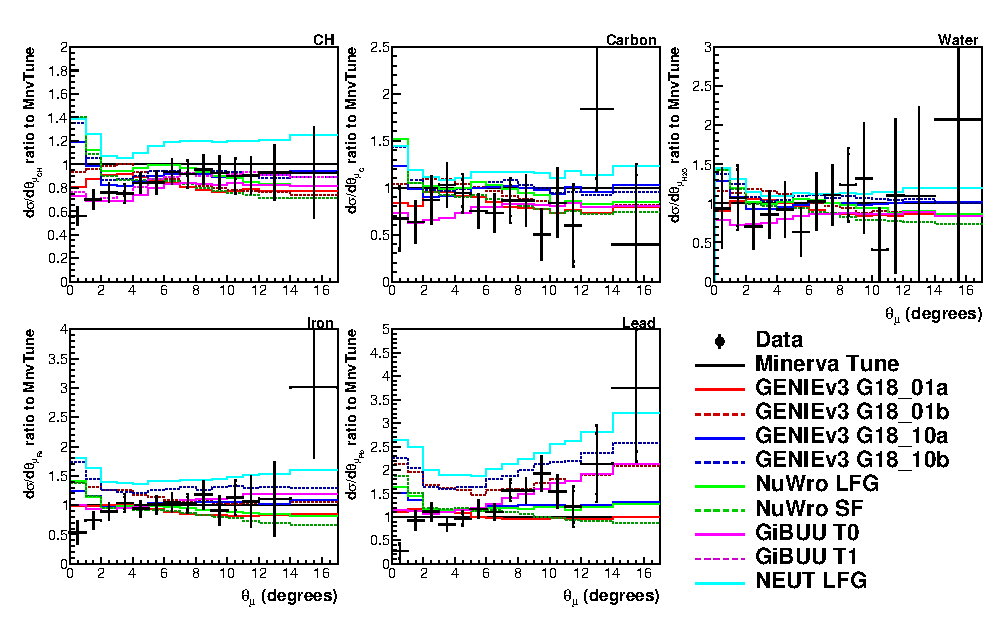
\includegraphics[width=\linewidth]{Figures/gencompare_ratio/mnvratio_muon_theta.eps}
    \caption{Ratio of absolute cross section measurements to the MINERvA tune for different targets as a function of $\theta_{\mu}$ and ratios of different model predictions to the MINERvA tune.}
    \label{fig:models_muon_theta_rat}
\end{figure}
\begin{figure}
    \centering
 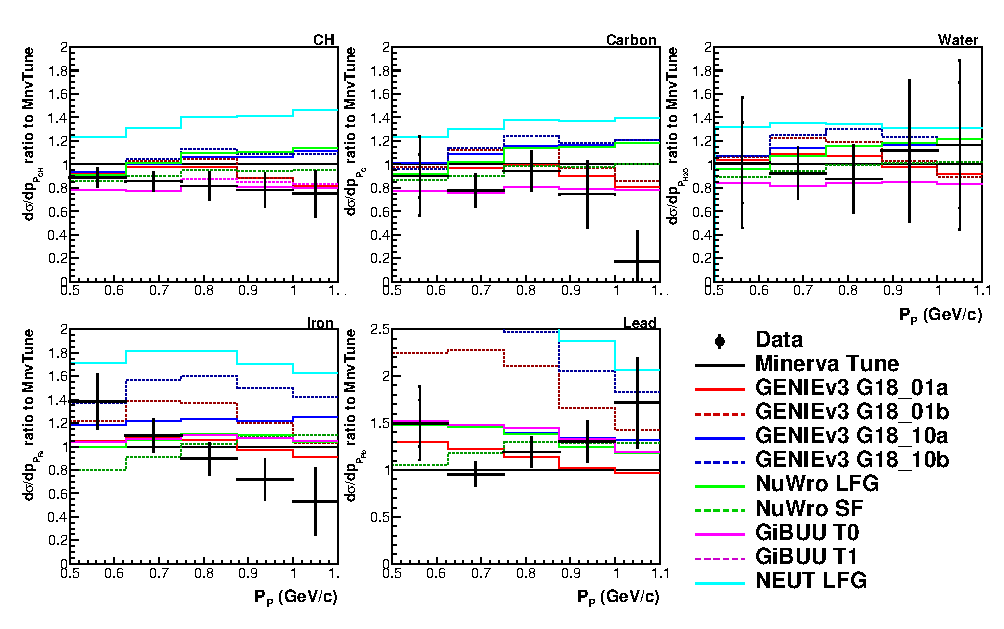
\includegraphics[width=\linewidth]{Figures/gencompare_ratio/mnvratio_proton_p.eps}
    \caption{Ratio of absolute cross section measurements to the MINERvA tune for different targets as a function of P$_{p}$ and ratios of different model predictions to the MINERvA tune.}
    \label{fig:models_proton_p_rat}
\end{figure}
\begin{figure}
    \centering
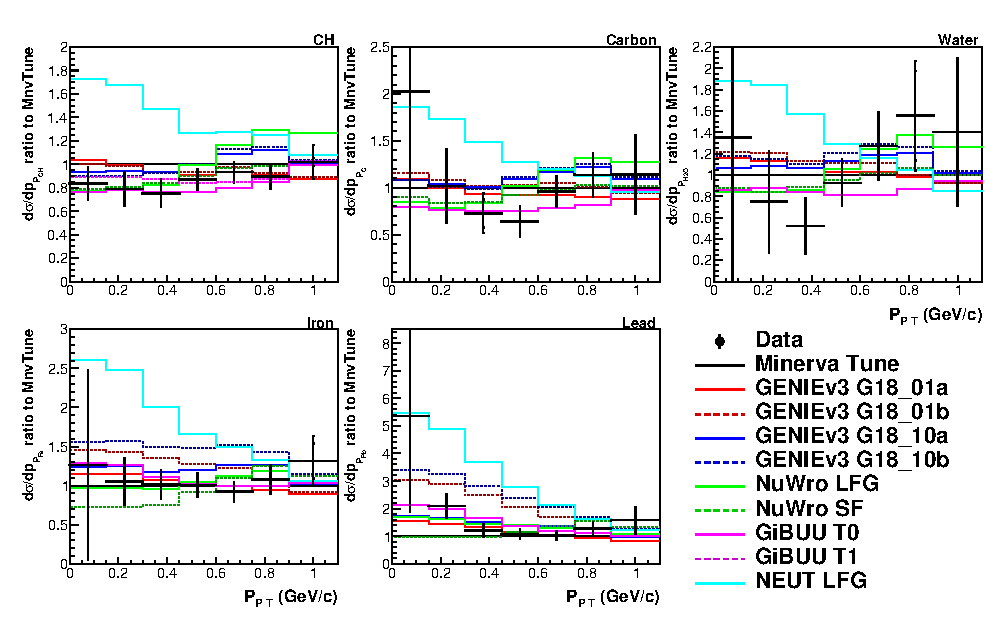
\includegraphics[width=\linewidth]{Figures/gencompare_ratio/mnvratio_proton_pt.eps}
    \caption{Ratio of absolute cross section measurements to the MINERvA tune for different targets as a function of P$_{p T}$ and ratios of different model predictions to the MINERvA tune.}
    \label{fig:models_proton_pt_rat}
\end{figure}
\begin{figure}
    \centering
    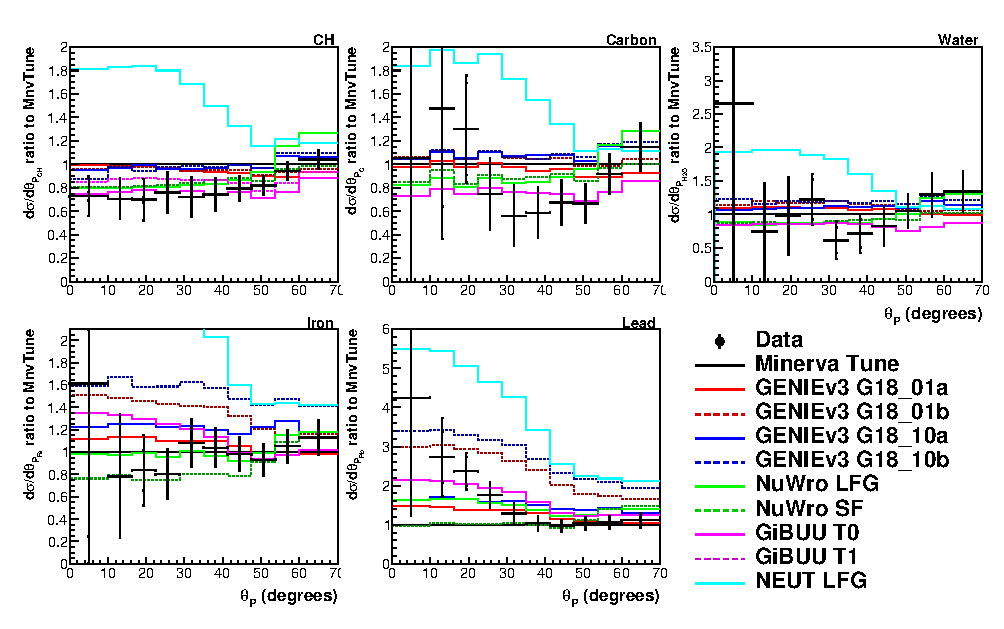
\includegraphics[width=\linewidth]{Figures/gencompare_ratio/mnvratio_proton_theta.eps}
    \caption{Ratio of absolute cross section measurements to the MINERvA tune for different targets as a function of $\theta_{p}$ and ratios of different model predictions to the MINERvA tune.}
    \label{fig:models_proton_theta_rat}
\end{figure}